\documentclass[cal1spr16Lectures.tex]{subfiles}
%\AtBeginSubsection{
%	\begin{frame}[allowframebreaks]{}
%	\begin{multicols}{2}
%	\tableofcontents[currentsubsection]
%	\end{multicols}
%	\end{frame}
%	}
	
\begin{document}

%\section[Week 4]{Week 4: 8-12 February}

% % %
\subsubsection{\bf Monday 8 February}
\begin{frame}[allowframebreaks]{Mon 8 Feb}
\begin{itemize}\footnotesize
\item EXAM 1 on Friday.  
\begin{itemize}\footnotesize
	\item Covers up to \S 3.1 (see the semester schedule of material on the course webpage). 
	\item \alert{You must attend your own lecture on exam day.}  
	\item CEA: Register with the CEA office for a time on 12 Feb, as close to your normal lecture time as possible.
	\item Look at old Wheeler exams to study.
	\url{comp.uark.edu/~ashleykw}
	\item Also look at Quiz and Drill solutions posted in MLP.
	\item Do the book problems.  Go to office hours or Calculus Corner to get feedback.
\end{itemize}	
\framebreak
\item Quizzes: 
\begin{itemize}
	\item Include drill instructor and time.
	\item Don't turn in the Quiz sheet with your work.
	\item No quiz again until next week.
	\item Drill Exercise Tues 16 Feb and Quiz 4 Thurs 18 Feb.
\end{itemize}
\framebreak
\item  Announcement: 

\alert{A student in this class requires a note-taker. If you are willing to upload your notes and plan to attend class on a REGULAR basis, please sign up via the CEA Online Services on the Center for Educational Access (CEA) website \url{http://cea.uark.edu}. On the CEA Online Services login screen, click on ``Sign Up as a Note-taker". At the end of the semester you will receive verification of 48 community service hours OR a \$50 gift card for providing class notes. All interested students are encouraged to sign up; preference may be given to volunteers seeking community service in an effort engage U of A students in community service opportunities. Please contact the Center for Educational Access at ceanotes@uark.edu if you have any questions.}

\end{itemize}
\end{frame}

% % %
\begin{frame}{}
\begin{exe} Let $f(x)=x^2-4$.  For $\epsilon=1$, find a value for $\delta>0$ so that 
\[|f(x)-12|<\epsilon \quad \text{whenever}\quad 0<|x-4|<\delta.\]
\end{exe}
In this example,  $\lim_{x \to 4}f(x)=12.$  
\end{frame}

% % %
\subsubsection{Book Problems}
% % %

% % %
\begin{frame}
\begin{block}{2.7 Book Problems} 1-7, 9-18 \end{block}
\end{frame}

% % %
\subsection[3.1 Introducing the Derivative]{\S 3.1 Introducing the Derivative}
% % %

% % %
\begin{frame}{\S 3.1 Introducing the Derivative}{}
{\bf Recall from Ch 2:}  We said that the slope of the tangent line at a point is the limit of the slopes of the secant lines as the points get closer and closer.
\begin{itemize}
\item slope of secant line:  $\dfrac{f(x)-f(a)}{x-a}$\ (average rate of change) 
\item slope of tangent line:  $\lim_{x \to a} \frac{f(x)-f(a)}{x-a}$\ (instantaneous rate of change)
\end{itemize}
\end{frame}

% % %
\begin{frame}
\centering{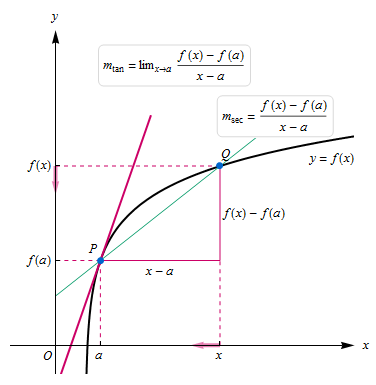
\includegraphics[scale=0.62]{pictures/lim}}
\end{frame}

% % %
\begin{frame}
\begin{exe} Use the relationship between secant lines and tangent lines, specifically the slope of the tangent line, to find the equation of a line tangent to the curve $f(x)=x^2+2x+2$ at the point $P=(1,5)$.
\end{exe}
\end{frame}

% % %
\begin{frame}{}
In the preceding exercise, we considered two points 
\vspace{-0.6pc}
\[P=\left(a,f(a)\right)\quad\text{and}\quad Q=\left(\alert{x},f(\alert{x})\right)\]
that were getting closer and closer together.

\vspace{2pc}
Instead of looking at the points approaching one another, we can also view this as the distance $h$ between the points approaching 0.  For 
\vspace{-0.5pc}
\[P=\left(a,f(a)\right)\quad\text{and}\quad Q=\left(\alert{a+h},f(\alert{a+h})\right),\]
\end{frame}

% % %
\begin{frame}
\begin{itemize}
\item slope of secant line:  
\[\frac{f(a+h)-f(a)}{(a+h)-a}= \dfrac{f(a+h)-f(a)}{h}\]
\item slope of tangent line:  
\[\lim_{h \to 0} \frac{f(a+h)-f(a)}{h}\]
\end{itemize}
\end{frame}

% % %
\begin{frame}
\centering{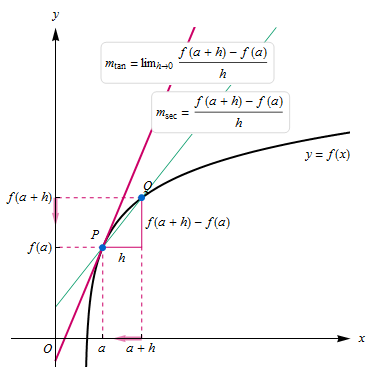
\includegraphics[scale=0.65]{pictures/limDef3_1}}
\end{frame}

% % %
\begin{frame}
\begin{exe} Find the equation of a line tangent to the curve $f(x)=x^2+2x+2$ at the point $P=(2,10)$. \end{exe}
\end{frame}

% % %
\subsubsection{Derivative Defined as a Function}
% % %

% % %
\begin{frame}{\small Derivative Defined as a Function}\footnotesize
The slope of the tangent line for the function $f$ is itself a function of $x$ (in other words, there is an expression where we can plug in any value $x=a$ and get the derivative at that point), called the derivative of $f$.
\begin{dfn} The {\bf derivative} of $f$ is the function 
\[f^{\prime}(x)=\lim_{h \to 0} \frac{f(x+h)-f(x)}{h},\]
provided the limit exists.  If $f^{\prime}(x)$ exists, we say $f$ is {\bf differentiable} at $x$.  If $f$ is differentiable at every point of an open interval $I$, we say that $f$ is differentiable on $I$. \end{dfn}
\end{frame}

% % %
\begin{frame}
\begin{exe} Use the definition of the derivative to find the derivative of the function $f(x)=x^2+2x+2$. \end{exe}
\end{frame}

% % %
\subsubsection{Leibniz Notation}
% % %

% % %
\begin{frame}{\small Leibniz Notation}
A standard notation for change involves the Greek letter $\Delta$. 
\[\frac{f(x+h)-f(x)}{h}=\frac{f(x+\Delta x)-f(x)}{\Delta x}=\frac{\Delta y}{\Delta x}.\]
Apply the limit:
\[f^{\prime}(x)=\lim_{\Delta x \to 0} \frac{f(x+\Delta x)-f(x)}{\Delta x}=\lim_{\Delta x \to 0} \frac{\Delta y}{\Delta x}=\alert{\frac{dy}{dx}}\]
\end{frame}

% % %
\subsubsection{Other Notation}
% % %

% % %
\begin{frame}{\small Other Notation}
The following are alternative ways of writing $f^{\prime}(x)$ (i.e., the derivative as a function of $x$):
\[\frac{dy}{dx}\qquad\frac{df}{dx} \qquad\frac{d}{dx}\left(f(x)\right) \qquad D_x (f(x)) \qquad y^{\prime}(x)\]
The following are ways to notate the derivative of $f$ evaluated at $x=a$:
\[f^{\prime}(a)\qquad y^{\prime}(a) \qquad \left. \frac{df}{dx} \right|_{x=a} \qquad \left. \frac{dy}{dx} \right|_{x=a}\]
\end{frame}

\end{document}